% \documentclass[CJKutf8, 10pt, handout]{beamer}
\documentclass[10pt,table]{beamer}
\usetheme[
%%% options passed to the outer theme
%    hidetitle,           % hide the (short) title in the sidebar
%    hideauthor,          % hide the (short) author in the sidebar
    hideinstitute,       % hide the (short) institute in the bottom of the sidebar
%    shownavsym,          % show the navigation symbols
%    width=2cm,           % width of the sidebar (default is 2 cm)
%    hideothersubsections,% hide all subsections but the subsections in the current section
%    hideallsubsections,  % hide all subsections
%    right                % right of left position of sidebar (default is right)
]{Aalborg}
  
% If you want to change the colors of the various elements in the theme,
% edit and uncomment the following lines.
% Change the bar and sidebar colors:
%\setbeamercolor{Aalborg}{fg=red!20,bg=red}
%\setbeamercolor{sidebar}{bg=red!20}
% Change the color of the structural elements:
%\setbeamercolor{structure}{fg=red}
% Change the frame title text color:
%\setbeamercolor{frametitle}{fg=blue}
% Change the normal text color background:
%\setbeamercolor{normal text}{bg=gray!6}
\setbeamercolor{normal text}{bg=white}

\usepackage[UTF8,noindent]{ctexcap}
\usepackage{color}
\usepackage{graphicx}
\usepackage{xcolor}
% 指定存储图片的路径(当前目录下的figures文件夹)
%\graphicspath{{figures/}}

\usepackage{fancybox}
\usepackage[utf8]{inputenc}
\usepackage[english]{babel}
\usepackage[T1]{fontenc}
% ... or whatever. Note that the encoding and the font should match.
% If T1 does not look nice, try deleting the line with the fontenc.
\usepackage{lmodern} %optional
\usepackage{listings}
\usepackage{wasysym}
\usepackage{tikz}
\usepackage{tikz-3dplot}



%%%%%%%% User Specified Commands %%%%%%%%
\setbeamercolor{alerted text}{fg=red!2!green!35!blue}
\newenvironment{boxalertenv}{\begin{altenv}%
  {\usebeamertemplate{alerted text begin}\usebeamercolor[fg]
    {alerted text}\usebeamerfont{alerted text}\colorbox{bg}}
  {\usebeamertemplate{alerted text end}}{\color{.}}{}}{\end{altenv}}
\newcommand<>{\boxalert}[1]{{%
  \begin{boxalertenv}#2{#1}\end{boxalertenv}%
}}

\def\hilite<#1>{%
  \temporal<#1>{\color{gray}}{\color{red!2!green!35!blue}}%
    {\color{blue!25}}}

% colored hyperlinks
\newcommand{\chref}[2]{%
  \href{#1}{{\usebeamercolor[bg]{Aalborg}#2}}
}

\definecolor{listinggray}{gray}{0.9}
\definecolor{lbcolor}{rgb}{0.9,0.9,0.9}
\lstset{
	language=C,
	captionpos=b,
	tabsize=4,
	frame=lines,
	keywordstyle=\color{blue},
	commentstyle=\color{darkgreen},
	stringstyle=\color{red},
	breaklines=true,
	showstringspaces=false,
	basicstyle=\footnotesize,
	emph={label}
	}

%%%%%%%% 设置字号 %%%%%%%%
\newcommand{\chuhao}{\fontsize{42pt}{\baselineskip}\selectfont}
\newcommand{\xiaochuhao}{\fontsize{36pt}{\baselineskip}\selectfont}
\newcommand{\yihao}{\fontsize{28pt}{\baselineskip}\selectfont}
\newcommand{\erhao}{\fontsize{21pt}{\baselineskip}\selectfont}
\newcommand{\xiaoerhao}{\fontsize{18pt}{\baselineskip}\selectfont}
\newcommand{\sanhao}{\fontsize{15.75pt}{\baselineskip}\selectfont}
\newcommand{\sihao}{\fontsize{14pt}{\baselineskip}\selectfont}
\newcommand{\xiaosihao}{\fontsize{12pt}{\baselineskip}\selectfont}
\newcommand{\wuhao}{\fontsize{10.5pt}{\baselineskip}\selectfont}
\newcommand{\xiaowuhao}{\fontsize{9pt}{\baselineskip}\selectfont}
\newcommand{\liuhao}{\fontsize{7.875pt}{\baselineskip}\selectfont}
\newcommand{\xiaoliuhao}{\fontsize{6.05pt}{\baselineskip}\selectfont}
\newcommand{\qihao}{\fontsize{5.25pt}{\baselineskip}\selectfont}

\AtBeginSection[]
{
\begin{frame}[shrink]

  \frametitle{目录}
  \CJKfamily{you}{\tableofcontents[%
 		currentsection, % causes all sections but the current to be shown in a semi-transparent way.
% 		currentsubsection, % causes all subsections but the current subsection in the current section to ...
% 		hideallsubsections, % causes all subsections to be hidden.
 		hideothersubsections, % causes the subsections of sections other than the current one to be hidden.
% 		part=, % part number causes the table of contents of part part number to be shown
%		pausesections, % causes a \pause command to be issued before each section. This is useful if you
% 		pausesubsections, %  causes a \pause command to be issued before each subsection.
% 		sections={ overlay specification },
  ]}

\end{frame}
}

\begin{document}


\title[PCA学习(二)]% optional, use only with long paper titles
{\erhao PCA学习(二)\\[2ex]}

\subtitle[OSS\ C\ SDK] %optional
{PCA证明及特征脸提取}

\author[王泽民] % optional, use only with lots of authors
{
\textcolor[rgb]{0.00, 0.41, 0.66}{王泽民\\[2ex]}
\textcolor[rgb]{0.00, 0.41, 0.66}{\texttt{691077364@qq.com}}
% \href{mailto:haipingf@gmail.com}{{\tt haipingf@gmail.com}}
}

% - Give the names in the same order as they appear in the paper.
% - Use the \inst{?} command only if the authors have different
%   affiliation. See the beamer manual for an example

%specify some optional logos
% placed in the upper left/right corner
\pgfdeclareimage[height=1.0cm]{mainlogo}{1.png} 
\logo{\pgfuseimage{mainlogo}}
% placed in the lower left/right corner if the \pgfuseimage{minilogo} command is
% uncommented in the \institute command below.
\pgfdeclareimage[height=0.3cm]{minilogo}{ict-logo-mini.pdf} 

\institute[
  {\pgfuseimage{minilogo}}\\ %insert a company or department logo
  School of Software,\\
  Chinese Academy of Sciences, Beijing
] % optional - is placed in the bottom of the sidebar on every slide
{%
\textcolor[rgb]{0.07, 0.31, 0.60}{
  \wuhao 软件学院\\[2ex]
  \xiaowuhao 中山大学}
  
  % there must be an empty line above this line - otherwise some unwanted space is added
  % between the university and the country (I do not know why;( )
}
% \date{\today}
\date{\textcolor[rgb]{0.00, 0.41, 0.46}{2014.10.30}}

% the titlepage
% the plain option removes the sidebar and header from the title page
\begin{frame}[plain] 
  \titlepage
\end{frame}
%%%%%%%%%%%%%%%%

% TOC
\begin{frame}{提纲}{}
 \CJKfamily{you}{\tableofcontents}
\end{frame}
%%%%%%%%%%%%%%%%%%%%%%%%%%%%%%%%%%%%%%%%%%%%%%%%%%%%%%%%%%%%
\section{PCA数学证明}
%%%%%%%%%%%%%%%%
\begin{frame}{}
在Ng的机器学习课上说关于PCA有9-10种数学解释\\
今天主要从两个角度:
     \begin{itemize}
     \hilite<1>  \item {最大化方差理论 }
    \hilite<2>  \item {最小化误差}
     \end{itemize}
\end{frame}

\subsection{最大化方差}
\begin{frame}
\frametitle{问题引出}
最好的k维特征是将n维样本点转换为k维后,每一维上的样本方差都很大\\
     比如下图有5个样本点:(已经做过预处理,均值为0,特征方差归一)
     \begin{center}
     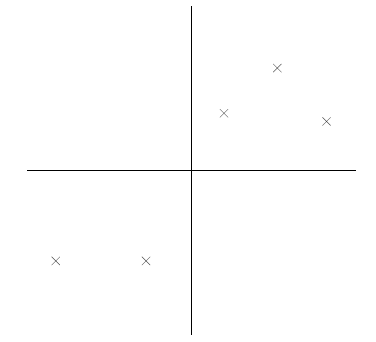
\includegraphics[width=0.6\textwidth]{max0.png}
     \end{center}
\end{frame}

\begin{frame}
  \begin{columns}[t]
  \column{0.5\textwidth}
\begin{figure}

  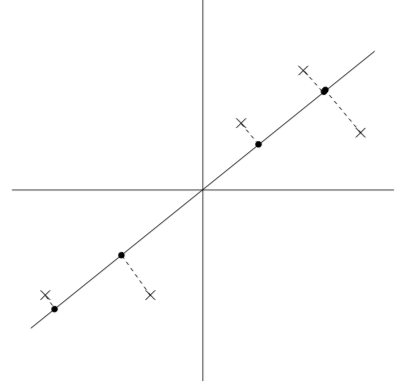
\includegraphics[width=\textwidth]{max1.png}
  \caption{此方向上投影方差较大}
  \end{figure}
  
  \pause
  \column{0.5\textwidth}
\begin{figure}
  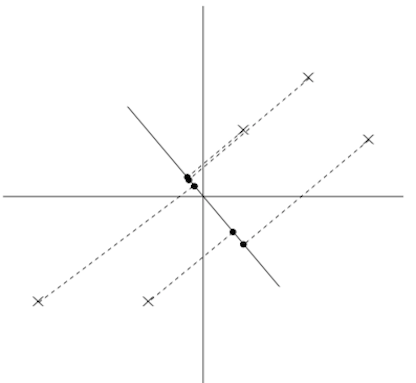
\includegraphics[width=\textwidth]{max2.png}
  \caption{此方向上投影方差较小}
  \end{figure}
  \end{columns}
\end{frame}

\definecolor{regular}{rgb}{.00,.785,.340}
\begin{frame}{投影}
\onslide<1->{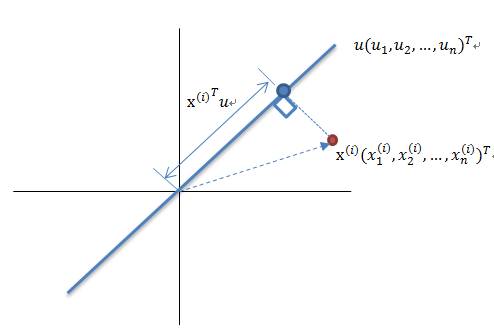
\includegraphics[width=0.8\textwidth]{max3.png} }
\only<1>{
 \begin{table}
\rowcolors[]{1}{regular!20}{regular!10}
\begin{tabular}{cc}

红色点 & 样例 \\
u  & 直线斜率,直线的方向向量(单位向量) \\
蓝色点 & 样例在u上的投影\\

  \end{tabular}
  \end{table} }
  \only<2>{
  这些样本点(样例)的每一维特征均值都为0,因此投影到u上的样本点(只有一个到原点的距离值)的均值仍然是0}
\end{frame}


\begin{frame}
 \[\begin{array}{l l l}
  Var(a)
           & =  & \frac{1}{m}\displaystyle{  \sum_{i=1}^m{(x^{(i)T}\mu)^2} }\\
           & =  &\frac{1}{m} \displaystyle{ \sum_{i=1}^m{(x^{(i)T}u)^T(x^{(i)T}u)}  }\\
           & = &\frac{1}{m}\displaystyle{  u^Tx^{(i)^T}x^{(i)}u }\\
           & = & \displaystyle{ u^{T}[\frac{1}{m}x^{(i)}x^{(i)T}]u}
  \end{array}\]
  
  记$$
  \Sigma = \frac{1}{m}x^{(i)}x^{(i)T}
  $$
\end{frame}


\begin{frame}
问题
$$\max \mu^T \Sigma \mu$$
$$st~ \mu^T\mu = 1$$
定义:\\
$$ L(\mu, \lambda) = \mu^T \Sigma \mu - \lambda(\mu^T\mu-1)$$
\end{frame}

\begin{frame}
\frametitle{拉格朗日乘子法}
是一种寻找变量受等值条件所限制的多元函数的极值的方法\\
先看一个二维的例子:\\
假设有函数:f(x, y),要求其极值.\\
且满足条件:\\
$ g\left( x,y \right) = c$\\


\end{frame}

\begin{frame}
\frametitle{拉格朗日乘子法}
\begin{center}
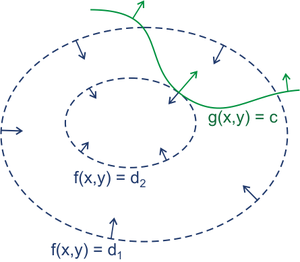
\includegraphics[width=0.5\textwidth]{lang.png}
\end{center} 
 \begin{table}
\rowcolors[]{1}{regular!20}{regular!10}
\begin{tabular}{cc}
绿线 & 约束g(x,y) = c的点的轨迹 \\
蓝线  & f的等高(值)线,$d_1<d_2$ \\
箭头 &斜率,和等高线的法线平行\\
  \end{tabular}
  \end{table}
\end{frame}


\begin{frame}
\begin{columns}[t]
  \column{0.5\textwidth}
  \center
  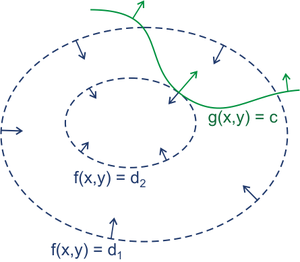
\includegraphics[width=0.7\textwidth]{lang.png} 
 
  
   \column{0.5\textwidth}
   \only<1>{
   想像我们沿着 g = c 的可行集走;因为大部分情况下 f 的等高线和 g 的可行集线不会重合,但在有解的情况下,这两条线会相交。想像此时我们移动 g = c 上的点,因为 f 是连续的方程,我们因此能走到$f \left( x, y \right)=d_n$更高或更低的等高线上,也就是说$d_n$可以变大或变小}
   
   \only<2>{只有当 g = c 和$f \left( x, y \right)=d_n$相切,也就是说,此时,我们正同时沿着 g = c 和$f \left( x, y \right)=d_n$走。这种情况下,会出现极值}
   
   \only<3>{
   用向量的形式来表达的话,我们说相切的性质在此意味着 f 和 g 的切线在某点上平行。此时引入一个未知标量$\lambda$,并求解:
\[  \nabla \Big[f \left(x, y \right) + \lambda \left(g \left(x, y \right) - c \right) \Big] = 0 \]
 且$\lambda \neq 0$}
 
 \end{columns}
\end{frame}

\begin{frame}
\frametitle{矩阵求导}
行向量$y^T$对列向量x求导:\\
注意1xM向量对$Nx 1$向量求导后是NxM矩阵\\
   将Y的每一列对x求偏导,将各列构成一个矩阵
   \[ 
   \begin{bmatrix}
 \frac{  \partial  y_1}{ \partial x_1 } &\dots &  \frac{  \partial  y_m}{ \partial x_1 } \\
 &\ddots &\vdots \\
 
 \frac{  \partial  y_1}{ \partial  x_n }&\dots &\frac{  \partial  y_m}{ \partial  x_n }
   \end{bmatrix}
   \]
   重要结论:

\[ \frac{dx^T} {dx} = I \]
\[ \frac{d(fg)}{dx}=(\frac{df^T}{dx})g+(\frac{dg}{dx})f^T \]
\end{frame}

\begin{frame}{求解}
$$ L(\mu, \lambda) = \mu^T \Sigma \mu - \lambda(\mu^T\mu-1)$$
对$\mu$求偏导:\\
\[ \nabla L = 2\Sigma \mu -2\lambda \mu = 0 \]
$\mu$就是特征向量,选取前k个特征值:\\
\[y^{(i)} =  
\begin{bmatrix}
\mu_1^{T}x^{(i)} \\
\mu_2^{T}x^{(i)} \\
\vdots \\
\mu_k^{T}x^{(i)}
\end{bmatrix} \]

\end{frame}
%%%%%%%%%%%%%%%%
\subsection{最小化误差}
\begin{frame}{最小化误差}
\only<1>{
\begin{center}
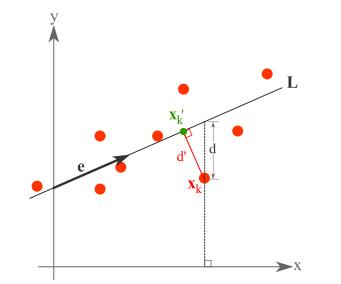
\includegraphics[width=5cm]{min0.png}
\end{center}
 假设有这样的二维样本点(红色点),本质是求直线,那么度量直线求的好不好,不仅仅只有方差最大化的方法。再回想我们最开始学习的线性回归等,目的也是求一个线性函数使得直线能够最佳拟合样本点,那么我们能不能认为最佳的直线就是回归后的直线呢?}
 
 \only<2>{
 \begin{columns}[t]
  \column{0.5\textwidth}
 \[  \begin{pmatrix}
  -1 & -1 & 0 & 2 & 0 \\
  -2 & 0 & 0 & 1 & 1
  \end{pmatrix} \]
  \center
  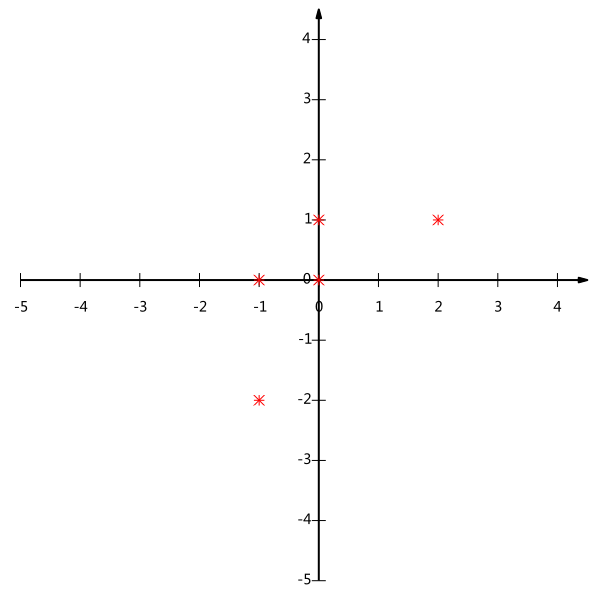
\includegraphics[width=\textwidth]{axis0.png}
  
  \column{0.5\textwidth}
  最小二乘法:
 \[ a =\frac{N\Sigma {xy}-\Sigma x \Sigma y}{N\Sigma{x^2}-(\Sigma x)^2}\]
解得斜率为$\frac23$\\

PCA: \\
解得斜率为1
  
 \end{columns}
 }
\end{frame}


\begin{frame}
\begin{columns}
\column{0.5\textwidth}
\begin{figure}
\center
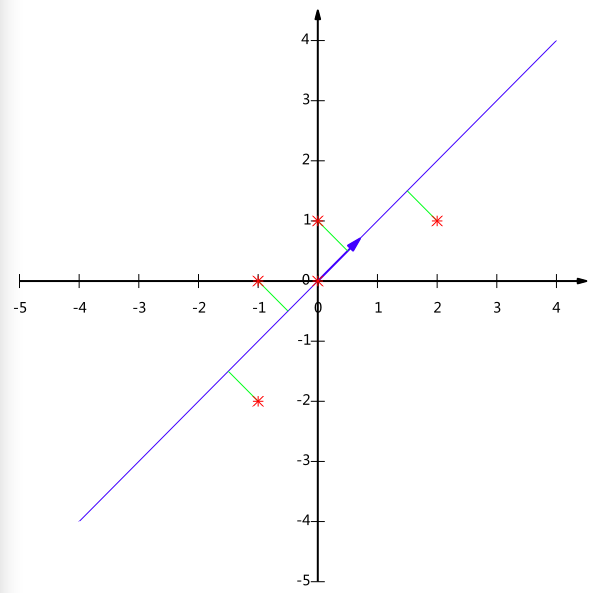
\includegraphics[width=\textwidth]{axis_ans.png}
\caption{PCA结果}
\end{figure}

\column{0.5\textwidth}
\begin{figure}
\center
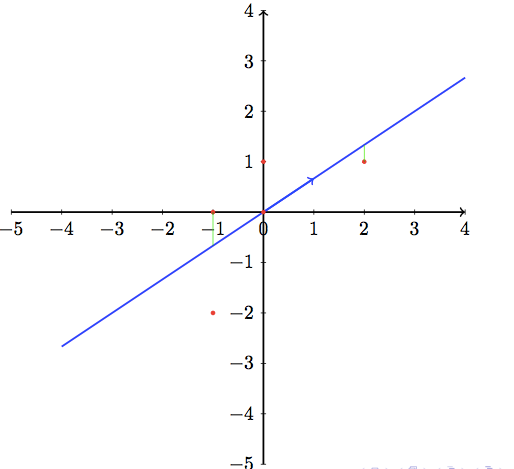
\includegraphics[width=\textwidth]{axis_ans2.png}
\caption{回归结果}
\end{figure}
\end{columns}
投影并不改变数据的分布
\end{frame}



\begin{frame}
令直线 L 穿越m(样本中心点),$\mathbf{w} $为其指向向量,且$ \Vert\mathbf{w}\Vert=1$\\直线 L 上的任一点可表示如下:

\[ \mathbf{x}=\mathbf{m}+c\mathbf{w},\]

其中 c 为一纯量,$\vert c\vert$ 代表$ \mathbf{x} $至$ \mathbf{m} $的距离。一旦 $\mathbf{w}$ 给定,我们可以用$ \mathbf{m}+c_k\mathbf{w} $来近似$ \mathbf{x}_k$,\\最佳的近似系数$ c_1,\ldots,c_n$ 必须最小化均方误差:
\[ \displaystyle \begin{aligned}  E_1(\{c_k\},\mathbf{w})&=\frac{1}{n-1}\sum_{k=1}^n\Vert(\mathbf{m}+c_k\mathbf{w})-\mathbf{x}_k\Vert^2\\  &=\frac{1}{n-1}\sum_{k=1}^n\Vert c_k\mathbf{w}-(\mathbf{x}_k-\mathbf{m}) \Vert^2\\  &=\frac{1}{n-1}\left(\sum_{k=1}^nc_k^2\Vert\mathbf{w}\Vert^2-2\sum_{k=1}^nc_k\mathbf{w}^T(\mathbf{x}_k-\mathbf{m})+\sum_{k=1}^n\Vert\mathbf{x}_k-\mathbf{m}\Vert^2\right).  \end{aligned} \]
\end{frame}


\begin{frame}
从几何上来看:\\
$c_k\mathbf{w} $即是离差$ \mathbf{x}_k-\mathbf{m}$ 在直线 L 的正交投影
%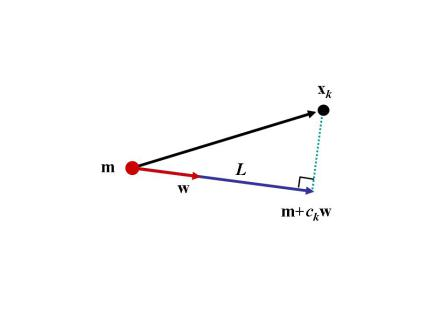
\includegraphics[width=\textwidth]{min1.jpg}
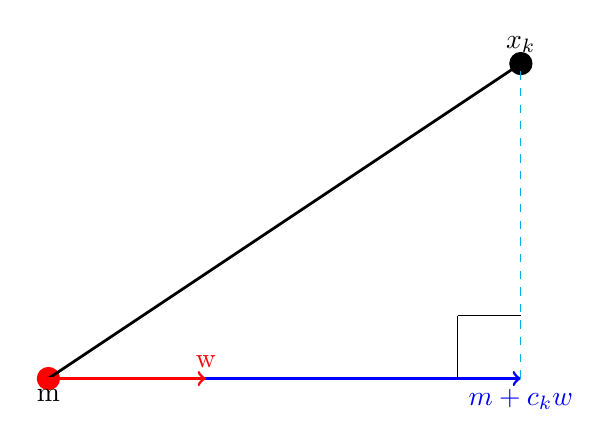
\begin{tikzpicture}[scale =2]
\filldraw [red] (0,0) circle(2pt);
  \filldraw  [black]  (3,2) circle(2pt);
\draw [line width =1pt,->] (0,0)node [anchor=north]{m}-- (3,2) node[anchor=south] {$x_k$};

\draw [blue,line width =1pt,->] (0,0)--(3,0)node [anchor = north]{$m+c_kw$};
\draw [red,line width =1pt,->] (0,0)--(1,0)node [anchor=south] {w};
\draw [cyan,dashed] (3,0)--(3,2);
\draw (2.6,0)--(2.6,0.4);
\draw (2.6,0.4)--(3.0,0.4);
\end{tikzpicture}

\end{frame}

\begin{frame}
\[c_k = \mathbf{w}^T(\mathbf{x}_k-\mathbf{m} )\]
利用这一关系进行化简:\\
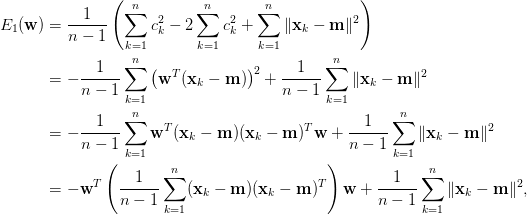
\includegraphics[width=\textwidth]{min2.png}\\
上面使用了$ \mathbf{w}^T(\mathbf{x}_k-\mathbf{m})=(\mathbf{x}_k-\mathbf{m})^T\mathbf{w}$令

$ \displaystyle  S=\frac{1}{n-1}\sum_{k=1}^n(\mathbf{x}_k-\mathbf{m})(\mathbf{x}_k-\mathbf{m})^T $

$ \sum_{k=1}^n\Vert\mathbf{x}_k-\mathbf{m}\Vert^2 $是一常数,所以最小化$ E_1(\mathbf{w}) $等价于最大化 $\mathbf{w}^TS\mathbf{w}$,这和之前转到同一个问题
\end{frame}



\begin{frame}
再来推广一下:
\[ \mathbf{x}=\mathbf{m}+z_{1}\mathbf{w}_1+\cdots+z_r\mathbf{w}_r \]

\[ \displaystyle  E_r\left(\{\mathbf{w}_j\}\right)=\sum_{k=1}^n\left\|\left(\mathbf{m}+\sum_{j=1}^rz_{kj}\mathbf{w}_j\right)-\mathbf{x}_k\right\|^2 \]
\end{frame}

\begin{frame}
化简:\\
\[ z_{kj} = w_j^T(x_k-m)\]
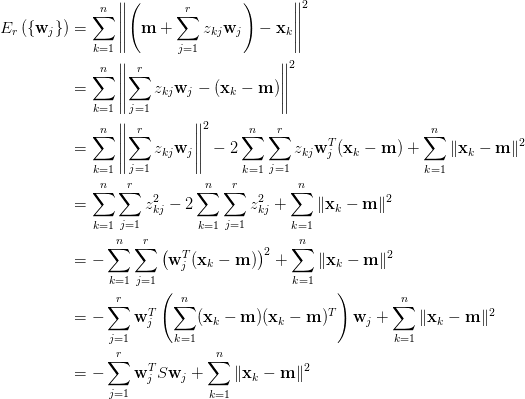
\includegraphics[width=\textwidth]{min3.png}
\end{frame}

\begin{frame}
 \[\displaystyle  \max_{\mathbf{w}_i^T\mathbf{w}_j=\delta_{ij}}\sum_{j=1}^r\mathbf{w}_j^TS\mathbf{w}_j \]
$\delta_{ij}=1$ 若 $i=j$,否则 $\delta_{ij}=0$ \\
定义

\[ \displaystyle  L\left(\{\mathbf{w}_j\},\{\mu_{ij}\}\right)=\sum_{j=1}^r\mathbf{w}_j^TS\mathbf{w}_j-\sum_{i=1}^r\sum_{j=1}^r\mu_{ij}(\mathbf{w}_i^T\mathbf{w}_j-\delta_{ij}) \]

\end{frame}

\begin{frame}
计算偏导数:
\[ \displaystyle  \frac{\partial L}{\partial \mathbf{w}_j}=2S\mathbf{w}_j-2\mu_{jj}\mathbf{w}_j-\sum_{i\neq j}(\mu_{ij}+\mu_{ji})\mathbf{w}_i=\mathbf{0},~~j=1,\ldots,r \]

对于$ i\neq j$,设 \[ \mu_{ij}+\mu_{ji}=0 
S\mathbf{w}_j=\mu_{jj}\mathbf{w}_j,~~j=1,\ldots,r \]
当$ \mathbf{w}_1,\ldots,\mathbf{w}_r$ 是样本协方差矩阵 S 的最大 r 个特征值$ \lambda_1,\ldots,\lambda_r $的对应 (标准正交) 特征向量时,目标函数 \[ \sum_{j=1}^r\mathbf{w}_j^TS\mathbf{w}_j=\sum_{j=1}^r\lambda_j\mathbf{w}_j^T\mathbf{w}_j=\sum_{j=1}^r\lambda_j \]有最大值
\end{frame}
%%%%%%%%%%%%%%%%


 \lstset{language=Matlab,basicstyle=\ttfamily,commentstyle=\ttfamily}
  \lstdefinestyle{Java}{delim=[il][\bfseries]{BB}}
  \definecolor{lightgray}{rgb}{.9,.9,.9}
  \lstset{backgroundcolor=\color{lightgray}}
\section{特征脸提取}

\subsection{代码}
\begin{frame}[fragile]{读取数据}
\alert<1>{Matlab:}
   \begin{footnotesize}
    
      \begin{lstlisting}[language=Matlab]
 numOfPic = 12;
picSize = 64; 
trainSet = zeros( numOfPic, 64*64 ); 
for i = 1 : numOfPic
     str=sprintf('res/face%05d.bmp',i);
     img = imread( str ); 
     img = imresize(img,[64,64]);	  
     img = double(img);
     trainSet(i,:) = img(:);
end
 \end{lstlisting}
     
  \end{footnotesize} 
  \pause
      \begin{itemize}
     \hilite<2>  \item {一行是一个数据,12个样本 }
    \hilite<3>  \item {每个样本64*64=4096维}
     \end{itemize}
\end{frame}
%%%%%%%%%%%%%%%%
\begin{frame}[fragile]{}
平均脸:\\
  \begin{lstlisting}[language=Matlab]
 meanValue = mean( trainSet );
trainSet_norm = bsxfun(@minus,trainSet, meanValue);
sigma = std(trainSet_norm); %每一列的标准差
trainSet_norm = bsxfun(@rdivide, trainSet_norm, sigma);
imwrite(uint8(reshape(meanValue, picSize, picSize)),'ans/mean.bmp');
  \end{lstlisting}
  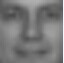
\includegraphics{mean.jpg}
\end{frame}
%%%%%%%%%%%%%%%%


\begin{frame}[fragile]{协方差矩阵与特征向量}
  \begin{lstlisting}[language=Matlab]
X = trainSet_norm;
[m, n] = size(X);

Cov = 1/m*X'*X;
[U ,S, V] =svd(Cov);

eigValue = diag(S);
AllSum = sum(eigValue);
cur_Sum = 0;
p =0;
while( cur_Sum/ AllSum < 0.9)
	p = p + 1;
        cur_Sum = sum(eigValue(1:p));
end;
  \end{lstlisting}
  p只有6
\end{frame}

%%%%%%%%%%%%%%%%%%%%%%%%%%%%%%%%%%%%%%%%%%%%%%%%%%%%%%%%%%%%


%%%%%%%%%%%%%%%%
\begin{frame}[fragile]{特征脸}{}
  \begin{lstlisting}[language=Matlab]
for i = 1:p
ef = P(:,i)';
minVal = min(ef);
ef =ef - minVal;
max_val = max(abs(ef));
ef = ef/max_val;  
Eigenface = reshape(ef,[64,64]);
str = sprintf('res/eigface%05d.bmp',i);
imwrite( Eigenface,str);
end
  \end{lstlisting}
\end{frame}


\begin{frame}{特征脸}
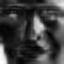
\includegraphics{c1.jpg}
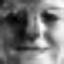
\includegraphics{c2.jpg}
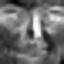
\includegraphics{c3.jpg}\\
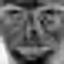
\includegraphics{c4.jpg}
\includegraphics{c5.jpg}
\includegraphics{c6.jpg}
\end{frame}

\begin{frame}[fragile]{测试与还原}
\begin{lstlisting}[language=Matlab]
testSet = zeros(4, 64*64);
for i = 3 :6
    str=sprintf('res/test%d.bmp',i);
    img =imread(str);
    img = double(img);
    testSet(i,:) = img(:);
end;
 \end{lstlisting}
 
\end{frame}
%%%%%%%%%%%%%%%%

\begin{frame}[fragile]{测试与还原}{}
\begin{lstlisting}[language=Matlab]
testNorm = bsxfun(@minus, testSet, meanValue);
Z = testNorm * P;
rc = Z * P';
for i = 3 : 6
   face = rc(i,:) + meanValue;
   rface = reshape(face, 64, 64);
   str = sprintf('res/test_re%d.bmp',i);
   imwrite(uint8(rface),str);
 
end;
 \end{lstlisting}
\end{frame}

\begin{frame}
\begin{columns}[t]
  \column{0.5\textwidth}
  \center
 
 \alert<1>{
  \begin{figure}
  \caption{测试图片}
  
\includegraphics[height=5cm]{12src.jpg} 
  \end{figure}
  }
 
 \pause
   \column{0.5\textwidth}
  \center
  \alert<2>{
   \begin{figure}
  \caption{还原结果}
  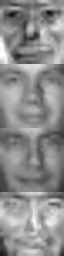
\includegraphics[height=5cm]{12re.jpg} 
   \end{figure}
  }
  \end{columns}
\end{frame}

%%%%%%%%%%%%%%%%

%%%%%%%%%%%%%%%%
\subsection{结果展示}
\begin{frame}{1200个样本}{平均脸}
\begin{columns}[t]
  \column{0.5\textwidth}
  \center

\includegraphics{meanex}
 \column{0.5\textwidth}
  看上去比较模糊,只是人脸的轮廓
  \end{columns}
\end{frame}

\begin{frame}{特征脸}{从19x19降到21}
我吧结果从19*19放大到64*64,看起来不太好\\
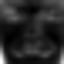
\includegraphics{eig/c1.jpg}
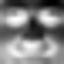
\includegraphics{eig/c2.jpg}
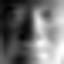
\includegraphics{eig/c3.jpg}
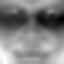
\includegraphics{eig/c4.jpg}\\
\includegraphics{eig/c5.jpg}
\includegraphics{eig/c6.jpg}
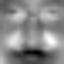
\includegraphics{eig/c7.jpg}
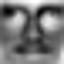
\includegraphics{eig/c8.jpg}
\end{frame}


\begin{frame}{Ng 在课堂上展示的特征脸}
1.从左到右是否被照亮\\
2.脸部明亮度\\
3. 脸部的阴影
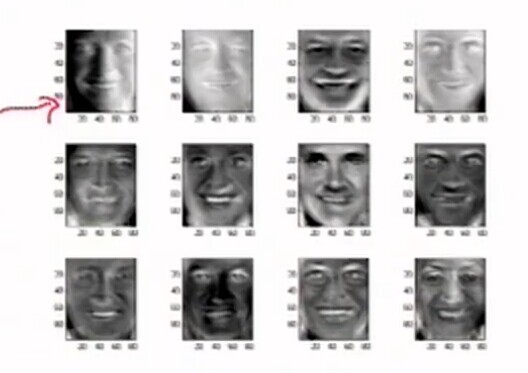
\includegraphics[width=\textwidth]{Ng.jpg}
\end{frame}

\begin{frame}{测试与还原}
\begin{columns}[t]
  \column{0.5\textwidth}
  \begin{figure}
  \center
  \caption{测试数据}
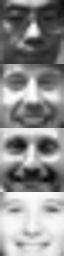
\includegraphics[height = 5cm]{src.jpg}
\end{figure}
\pause
 \column{0.5\textwidth}
 \begin{figure}
  \center
  \caption{还原结果}
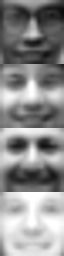
\includegraphics[height=5cm]{re.jpg}
\end{figure}
\end{columns}
\end{frame}
%%%%%%%%%%%%%%%%







\end{document}
